\documentclass[
% -- opções da classe memoir --
12pt,				% tamanho da fonte
openright,			% capítulos começam em pág ímpar (insere página vazia caso preciso)
oneside,			% para impressão em recto e verso. Oposto a oneside
a4paper,			% tamanho do papel.
% -- opções da classe abntex2 --
% chapter=TITLE,		% títulos de capítulos convertidos em letras maiúsculas
% section=TITLE,		% títulos de seções convertidos em letras maiúsculas
% subsection=TITLE,	% títulos de subseções convertidos em letras maiúsculas
% subsubsection=TITLE,% títulos de subsubseções convertidos em letras maiúsculas
% -- opções do pacote babel --
english,			% idioma adicional para hifenização
french,				% idioma adicional para hifenização
spanish,			% idioma adicional para hifenização
brazil,				% o último idioma é o principal do documento
]{abntex2}


% ---
% PACOTES
% ---

% ---
% Pacotes fundamentais
% ---
\usepackage{lmodern}			% Usa a fonte Latin Modern
\usepackage[T1]{fontenc}		% Selecao de codigos de fonte.
\usepackage[utf8]{inputenc}		% Codificacao do documento (conversão automática dos acentos)
\usepackage{indentfirst}		% Indenta o primeiro parágrafo de cada seção.
\usepackage{color}				% Controle das cores
\usepackage{graphicx}			% Inclusão de gráficos
\usepackage{microtype} 			% para melhorias de
% justificação
\usepackage{amsmath}
% ---

% ---
% Pacotes de citações
% ---
\usepackage[brazilian,hyperpageref]{backref}	 % Paginas com as citações na bibl
\usepackage[alf]{abntex2cite}	% Citações padrão ABNT


% ---
% Pacotes adicionais, usados no anexo do modelo de folha de identificação
% ---
% \usepackage{multicol}
% \usepackage{multirow}
% ---

% ---
% Pacotes adicionais, usados apenas no âmbito do Modelo Canônico do abnteX2
% ---
% \usepackage{lipsum}				% para geração de dummy text
% ---


% ---
% CONFIGURAÇÕES DE PACOTES
% ---

\usepackage{enumitem}
\setlist{nolistsep}

% ---
% Configurações do pacote backref
% Usado sem a opção hyperpageref de backref
\renewcommand{\backrefpagesname}{Citado na(s) página(s):~}
% Texto padrão antes do número das páginas
\renewcommand{\backref}{}
% Define os textos da citação
\renewcommand*{\backrefalt}[4]{
  \ifcase #1 %
  Nenhuma citação no texto.%
  \or
  Citado na página #2.%
  \else
  Citado #1 vezes nas páginas #2.%
  \fi}%
% ---

% ---
% Informações de dados para CAPA e FOLHA DE ROSTO
% ---
\titulo{Minicurso de \LaTeX}
\autor{Aluno: Pedro G. Branquinho \\ Orientadora: Katia Cristiane
  Gandolpho Candioto}
\local{Lorena, São Paulo}
\data{\today}%13 de Fevereiro de 2020}
\instituicao{%
  Universidade de São Paulo - USP \\
  Escola de Engenharia de Lorena
  \par
  LabEEL - DEMAR
  \par
  Projeto de Bolsa PUB}
\tipotrabalho{Relatório técnico}
% O preambulo deve conter o tipo do trabalho, o objetivo,
% o nome da instituição e a área de concentração
% \preambulo{Relato da elaboração e progresso do minicurso de \LaTeX}
% ---

% ---
% Configurações de aparência do PDF final

% alterando o aspecto da cor azul
\definecolor{blue}{RGB}{41,5,195}

% informações do PDF
\makeatletter
\hypersetup{
  % pagebackref=true,
  pdftitle={\@title},
  pdfauthor={\@author},
  pdfsubject={\imprimirpreambulo},
  pdfcreator={LaTeX with abnTeX2},
  pdfkeywords={abnt}{latex}{abntex}{abntex2}{relatório técnico},
  colorlinks=true,       		% false: boxed links; true: colored links
  linkcolor=blue,          	% color of internal links
  citecolor=blue,        		% color of links to bibliography
  filecolor=magenta,      		% color of file links
  urlcolor=blue,
  bookmarksdepth=4
}
\makeatother
% ---

% ---
% Espaçamentos entre linhas e parágrafos
% ---

% O tamanho do parágrafo é dado por:
\setlength{\parindent}{0.8cm}

% Controle do espaçamento entre um parágrafo e outro:
\setlength{\parskip}{0.2cm}  % tente também \onelineskip

% ---
% compila o indice
% ---
\makeindex
% ---

% ----
% Início do documento
% ----
\begin{document}

% Seleciona o idioma do documento (conforme pacotes do babel)
% \selectlanguage{english}
\selectlanguage{brazil}

% Retira espaço extra obsoleto entre as frases.
\frenchspacing

% ----------------------------------------------------------
% ELEMENTOS PRÉ-TEXTUAIS
% ----------------------------------------------------------
% \pretextual

% ---
% Capa
% ---
\imprimircapa
% ---

% ---
% RESUMO
% ---

% resumo na língua vernácula (obrigatório)
\setlength{\absparsep}{18pt} % ajusta o espaçamento dos parágrafos do resumo
\begin{resumo}
  Com o intuito de capacitar os alunos da instituição EEL-USP a
  utilizarem da ferramenta \LaTeX{} para tipografia, propôs-se um programa
  de ensino, em formato de minicurso, com uso de apostila didática e vídeos. O
  \LaTeX, é uma linguagem markdown de formatação de documentos. E se especializa em reproduzir trabalhos científicos, bem
  como ser fielmente reprodutível, quanto a seus documentos. O curso focou no
  ensino da ferramenta, com pacotes específicos para formatação em
  acordo com as normas ABNT, e os modelos canônicos do pacote. Também,
  foi ministrada aulas sobre a formatação de apresentações. Os alunos,
  também, foram capacitados a expandir seu conhecimentos, pois,
  aprenderam sobre pacotes essenciais, como o Tikz, o qual permite
  entender diversos pacotes do CTAN - o repositório oficial do \LaTeX.

  \noindent
  \textbf{Palavras-chaves}: minicurso. latex. modelos canônicos ABNT. capacitação.

\end{resumo}
% ---


% ---
% inserir o sumario
% ---
\pdfbookmark[0]{\contentsname}{toc}
\tableofcontents*
% ---


% ----------------------------------------------------------
% ELEMENTOS TEXTUAIS
% ----------------------------------------------------------
\textual

% ----------------------------------------------------------
% Introdução (exemplo de capítulo sem numeração, mas presente no Sumário)
% ----------------------------------------------------------
\chapter[Introdução]{Introdução}
% \addcontentsline{toc}{chapter}{Introdução}

O \LaTeX, um sistema de produção textual computacional, surgiu para
sistematizar toda a tipografia de documentos por meio digital. É
reconhecido, largamente, em formatação de linguagem matemática, e
produção documental científicas; documentos multilinguísticos; e,
especialmente, produções longas e complexas, como teses
\cite{ignat2005}

Por meio de uma sistematização localizada, por via de códigos, há uma
regularidade, previsibilidade, e reprodutividade superior em relação a
programas do tipo WYSIWYG, ``What You See Is What You Get'' - o que se
visualiza é o que se reproduz. Um exemplo desse paradigma é o software
Word, o qual é propriedade privada da Microsoft.

Além do mais, por ser um programa amplamente desenvolvido pela
comunidade como linguagem open source, ganha-se qualidade na
reutilização e evolução linguística dos usuários-desenvolvedores
\cite{goossens1994}. Pois, um arquivo, template, pacote, ou classe,
pode ser reutilizado, uma vez criado, para a resolução de problemas
recorrentes à comunidade. Desta forma, advém pacotes como o abnTeX,
desenvolvido pela equipe \abnTeX, CPAI - UnB, no Centro de Pesquisa em
Arquitetura de Informação. O pacote se compraz de ferramentas, e
modelos canônicos feitos estritamente sob às normas ABNT, os quais
podem ser utilizados e adaptados a todas instituições brasileiras que
siga as normas.


\section{Objetivo}

Por meio de minicurso profissionalizante, objetiva-se ensinar alunos da
EEL-USP a usarem a linguagem markup, \LaTeX. Assim, colaborando para
aumento do potencial dos alunos em reproduzir materiais tipografados
científicos de alto nível. Sejam eles, artigos, apresentações, livros,
relatórios, cartazes ou pôsteres.

Por conseguinte, objetivo do projeto é de ministrar três aulas de um minicurso de
\LaTeX, para alunos de graduação da EEL, explanando sobre a filosofia,
metodologia, e técnicas de produção de relatórios, teses, artigos, e
cartazes gráficos, como pôsters, por meio de pacotes essências do
\LaTeX, os quais permitem a elaboração e compreensão de qualquer
documento ou pacote mais avançado o qual o aluno venha a aprender ou utilizar.

\chapter{Revisão Bibliográfica}

\section{O \LaTeX}

O \LaTeX{} foca na separação das tarefas constituintes da produção de um
documento. A linguagem separa as tarefas de formatação do texto, da
escrita de seu conteúdo. Desta forma, o usuário concentra-se
exclusivamente em seu conteúdo - o que vai escrever -, em um
estágio da escrita do texto. E, na formatação de sua aparência, em
outro momento.

Assim, ganha-se em
qualidade de produção. Bem como, total autonomia sob o documento, pois
a programação da disposição gráfica dos elementos textuais depende apenas do usuário, e
pode ser indefinidamente extensível - isto é, modificada indefinidamente, a partir dos
comportamentos padrões dos pacotes utilizados -, por ser \textit{open source}. O sistema tipográfico de \LaTeX{} - o
\TeX{} - já chegou a ser considerado o sistema digital de
tipografia mais sofisticado que existe, devido a essa paradigma de
programação funcional, \textit{bottom-up} \cite{haralambous2007}.

O \LaTeX, tecnicamente, é a junção do sistema de tipografia \TeX,
inventado por Donald Knuth, para tipografia de alto nível
\cite{knuth1986}; com os poderosos macros que facilitam a extensão do programa \TeX, a qual damos o nome de
\LaTeX. O \LaTeX{} foi inicialmente desenvolvido por Leslie Lamport, com
seus pacotes fundamentais de formatação \cite{lamport1994}. O \LaTeX,
por conseguinte, não é somente uma linguagem de tipografia de alto
nível, mas também um conjunto de macros para facilitar a tipografia em
si. Qualifica-se, assim, como um sistema de preparação de documentos;
uma linguagem markup de domínio específico.

\section{Classe Canônica ABNT de produção científica}

Documentos sob os requisitos das normas ABNT (Associação Brasileira de Normas
Técnicas) para elaboração de documentos técnicos e científicos
brasileiros - como artigos científicos, relatórios técnicos, trabalhos
acadêmicos, como teses, dissertações, projetos de pesquisa e outros
documentos do gênero \cite{abntex2012} - é ao que se chama classe
canônica ABNT.

\begin{citacao}
  Os documentos indicados tratam-se de “Modelos Canônicos”, ou seja,
  de modelos que não são específicos a nenhuma universidade ou instituição, mas
  que implementam exclusivamente os requisitos das normas da ABNT, Associação
  Brasileira de Normas Técnicas. \cite[Cap. 1]{araujoclasse}
\end{citacao}

\clearpage

As normas as quais prescrevem o modelo canônico são:

\begin{itemize}
\item \textbf{ABNT NBR 6022:2018:} Informação e documentação -
  Artigo em publicação periódica científica - Apresentação.
\item \textbf{ABNT NBR 6023:2002:} Informação e documentação -
  Referência - Elaboração.
\item \textbf{ABNT NBR 6024:2012:} Informação e documentação -
  Numeração progressiva das secções de um documento - Apresentação.
\item \textbf{ABNT NBR 6027:2012:} Informação e documentação -
  Sumário - Apresentação.
\item \textbf{ABNT NBR 6028:2003:} Informação e documentação -
  Resumo - Apresentação.
\item \textbf{ABNT NBR 6029:2006:} Informação e documentação -
  Livros e folhetos - Apresentação.
\item \textbf{ABNT NBR 6034:2004:} Informação e documentação -
  Índice - Apresentação.
\item \textbf{ABNT NBR 10520:2002:} Informação e documentação -
  Citações.
\item \textbf{ABNT NBR 10719:2015:} Informação e documentação -
  Relatórios técnicos e/ou científico - Apresentação.
\item \textbf{ABNT NBR 14724:2011:} Informação e documentação -
  Trabalhos acadêmicos - Apresentação.
\item \textbf{ABNT NBR 15287:2011:} Informação e documentação -
  Projeto de pesquisa - Apresentação.
\end{itemize}

% \clearpage
\section{abnTeX}

A classe abnTeX foi criado para suprir as necessidades de
formatações, em padrão ABNT. E, por conseguinte, auxiliar o aumento
do nível de produção nacional. De acordo com o autor,

\begin{citacao}
  Dentre as características de qualidade de trabalhos acadêmicos (teses, dissertações e
  outros do gênero), de artigos científicos, de relatórios técnicos e de livros e folhetos,
  ao lado da pertinência do tema e dos aspectos relativos ao conteúdo abordado no
  trabalho, consta também o resultado da edição final e as características de
  forma e de estruturação dos documentos. Desse modo, a existência de um modelo
  e de ferramentas que atendam às normas brasileiras de elaboração de trabalhos
  acadêmicos, artigos científicos e relatórios técnicos propostas pela Associação
  Brasileira de Normas Técnicas (ABNT) são recursos básicos para o aprimoramento
  da qualidade geral dos trabalhos acadêmicos nacionais.

  É com esse intuito que o abn\TeX2 é apresentado à comunidade acadêmica brasileira:
  o de ser um instrumento de aperfeiçoamento da qualidade dos textos produzidos.
  O abnTEX2 surge para se somar ao já vasto universo de ferramentas LATEX, porém
  que é escasso em utilitários específicos para trabalhos brasileiros. \cite[2.1]{araujoclasse}
\end{citacao}

O pacote, para se tornar parte do corpo oficial de pacotes \LaTeX, foi
desenvolvido desde 2001, até 2013. E, hoje, é mantida pela comunidade
de software livre. Seu acesso à atual distribuição oficial pode ser
feita em \url{https://www.ctan.org/pkg/abntex2}. CTAN - Comprehensive TEX Archive Network - é o site
repositório dos pacotes ``oficiais'' do \LaTeX.

Assim, pela utilização de pacotes de formatação abnTeX2, o aluno
precisa apenas focar no texto, e material da pesquisa - pois a
formatação é automática. Por conseguinte,
aumenta-se as chances de melhorar a qualidade de produção de trabalhos
acadêmicos, que é base da filosofia da linguagem.

\section{CTAN}

CTAN é um repositório de pacotes do de \TeX. Todos os pacotes
fundamentais os quais constituem o \LaTeX podem ser encontrados no
CTAN. Ademais, todos os pacotes são documentados, integralmente, e
postados nesse repositório. Todas as imagens, por exemplo, \autoref{im:1},
\autoref{im:2}, \autoref{im:3}, \autoref{im:4}, podem ser encontradas
na documentação do Tikz, bem como os códigos que as produzem. Assim,
também é a documentação de outros pacotes - eles apresentam seus
comandos e os explicam como utilizar e os modular.

Os pacotes são mantidos pela comunidade. E, qualquer usuário pode se
tornar um desenvolvedor. Em fato, quando se faz modelos, e os
compartilha, como é comum em outros sites-repositórios, como o
\href{https://www.overleaf.com/}{Overleaf}, é um dos primeiros passos
para se crear um novo pacote, pois é uma extensão personificada das
funcionalidade de outros pacotes.

Antes de 1991, não existiam repositórios de pacotes de \TeX{}. No
intuito de unificar um ambiente em que pudesse se encontrar a maioria
dos pacotes existentes e gratuitos de \TeX{}, o CTAN surgiu
\cite{greenwade1993comprehensive}.

%\clearpage
\section{Beamer}

Desenvolvido pela comunidade, Beamer não é a primeira, porém, o mais
utilizado pacote para produção de slides e apresentações. Seus
desenvolvedores, iniciais, foram Louis Stuart, Till Tantau, Joseph
Wright, e Vedran Miletc \cite{tantau2010}. Por mais que estes sejam os principais
desenvolvedores, Beamer é um pacote livre e aberto, como o \LaTeX, em
si. Isto é, toda a comunidade usuária é também desenvolvedora do
pacote.


Desta forma, é um pacote extensivamente trabalhado para
produção de apresentações, disponível em diversas formatações
canônicas. A \autoref{im:10} apresenta dois exemplos de slides feitos
com Beamer, encontrados na internet.

\begin{figure}[!htb]
  \caption{\label{im:10} Exemplos de Slides Produzidos com Beamer}
  \begin{center}
    \includegraphics[width=0.45\linewidth]{./Imagens/beamer.png}
    \includegraphics[width=0.45\linewidth]{./Imagens/beamer2.jpg}
  \end{center}
  \legend{Fonte: \href{https://martin-thoma.com/author/martin-thoma/}{\cite{martin2013}}}
\end{figure}



\section{Tikz}

Tikz é um pacote essencial para manusear e crear imagens com
Postscript, por meio da linguagem \TeX. Com essa ferramenta, pode-se
fazer diagramas, gráficos, desenhos. Ele é um dos pacotes fundamentais
do \LaTeX{} \cite{lamport1994}. As imagens - \autoref{im:1}, \autoref{im:2},
\autoref{im:3}, \autoref{im:4}, \autoref{im:5}, \autoref{im:6}  - apresentam explanações de
código/resultado encontrados na documentação oficial do pacote \href{http://linorg.usp.br/CTAN/graphics/pgf/base/doc/pgfmanual.pdf}{Tikz}.

\begin{figure}[!htb]
  \caption{\label{im:1} Imagens escritas com Tikz, geometria}
  \begin{center}
    \includegraphics[width=\linewidth]{./Imagens/3.png}
  \end{center}
  \legend{Fonte:
    \href{http://linorg.usp.br/CTAN/graphics/pgf/base/doc/pgfmanual.pdf}{Manual
      Tikz, CTAN}}
\end{figure}

\begin{figure}[!htb]
  \caption{\label{im:2} Imagens escritas com Tikz, grafos}
  \begin{center}
    \includegraphics[width=\linewidth]{./Imagens/1.png}
  \end{center}
  \legend{Fonte:
    \href{http://linorg.usp.br/CTAN/graphics/pgf/base/doc/pgfmanual.pdf}{Manual
      Tikz, CTAN}}
\end{figure}
%% \begin{figure}[!htb]
%%   \caption{\label{im:3} Imagens escritas com Tikz, gráficos}
%%   \begin{center}
%%     \includegraphics[width=0.47\linewidth, \height=0.4\paperheight]{./Imagens/2.png}
%%     \includegraphics[width=0.47\linewidth, \height=0.4\paperheight]{./Imagens/6.png}
%%   \end{center}
%%   \legend{Fonte:
%%     \href{http://linorg.usp.br/CTAN/graphics/pgf/base/doc/pgfmanual.pdf}{Manual
%%       Tikz, CTAN}}
%% \end{figure}

\begin{figure}[!htb]
  \caption{\label{im:3} Imagens escritas com Tikz, gráficos}
  \begin{center}

    \includegraphics[width=\linewidth, \height=0.4\paperheight]{./Imagens/6.png}
  \end{center}
  \legend{Fonte:
    \href{http://linorg.usp.br/CTAN/graphics/pgf/base/doc/pgfmanual.pdf}{Manual
      Tikz, CTAN}}
\end{figure}

\begin{figure}[!htb]
  \caption{\label{im:4} Imagens escritas com Tikz, gráficos}
  \begin{center}
    \includegraphics[width=\linewidth, \height=0.4\paperheight]{./Imagens/2.png}
  \end{center}
  \legend{Fonte:
    \href{http://linorg.usp.br/CTAN/graphics/pgf/base/doc/pgfmanual.pdf}{Manual
      Tikz, CTAN}}
\end{figure}



\begin{figure}[!htb]
  \caption{\label{im:5} Imagens escritas com Tikz, representação da Luz}
  \begin{center}
    \includegraphics[width=\linewidth]{./Imagens/4.png}
  \end{center}
  \legend{Fonte:
    \href{http://linorg.usp.br/CTAN/graphics/pgf/base/doc/pgfmanual.pdf}{Manual
      Tikz, CTAN}}
\end{figure}


\begin{figure}[t]
  \caption{\label{im:6} Imagens escritas com Tikz, representação de um
    arbusto}
  \begin{center}
    \includegraphics[width=\linewidth]{./Imagens/5.png}
  \end{center}
  \legend{Fonte:
    \href{http://linorg.usp.br/CTAN/graphics/pgf/base/doc/pgfmanual.pdf}{Manual
      Tikz, CTAN}}
\end{figure}

\clearpage



\chapter{Materiais e Métodos}

O planejamento do minicurso seguiu as seguintes etapas:

\begin{enumerate}
\item Determinação do local/ambiente a serem ministradas as aulas presenciais e a distância;
\item Capacidade de vagas para as aulas;
\item Datas para realização das aulas;
\item Definição de temas e carga horária para cada aula;
\item Recursos e datas para divulgação e inscrição.
\item Elaboração de materiais e atividades para execução do curso;
\item Recursos para administração do minicurso;
\item Execução das aulas;
\item Validação da participação dos alunos;
\item Emissão de certificados.
\end{enumerate}

Porém, quando houve o anúncio da quarentena, pela USP, devido ao
Covid-19, planejou-se um novo cronograma e escolheu-se as plataformas,
para aulas à distância.

Decidiu-se por aulas disponibilizadas no Youtube, e encontros pela
plataforma Google Meet.

\section{Sediação}
O curso foi idealizado para até quarenta alunos. Procurou-se uma sala
que os comportasse, bem como tivesse os devidos equipamentos
eletrônicos para sediar apresentações.

Por fim, no entanto, as aulas foram gravadas e disponibilizadas no
Youtube. Foi, ademais, dadas aulas de revisão e dúvidas, pela
plataforma Google Meet. Da mesma forma, a disponibilidade também foi
readequada às condições; abriu-se vagas para um número de até cem
alunos. Pois, não havia a limitação de espaço físico.

\section{Data}
Procurou-se fazer escolha de datas que maximizassem a aderência, e
notoriedade do curso. Levou-se em conta, também, o calendário oficial
da USP, do semestre letivo.

\section{Definição dos temas}

As divisões de aula do curso foram feitas, esquematicamente, em nível
progressivo de complexidade e abstração, requerida para se produzir
documentos com alocação de imagens e modulações, como apresentações e pôsteres.

Procurou-se, para a escolha dos tópicos, e partição das aulas,
entender qual eram as necessidades dos alunos, quanto a produção
acadêmicos. Ao mesmo tempo, o curso foi projetado de forma a maximizar o
aprendizado sistemático do assunto.  Determinou-se que, tanto a
formatação sob as normas ABNT, como a formatação de apresentações de slides eram essenciais.

\section{Divulgação}

Procurou-se determinar quais eram os canais mais populares, e com
maiores retornos de público, para se divulgar. Bem como alocar a
divulgação em datas estratégias.

%E sobre os criterios de carga horária, avaliação, execução e conclusão com emissão dos certificados?
%Também não escreveu sobre as inscrições....

\section{Carga horária}
Para cada aula, foi alocada duas horas aula. Duas a quatro horas para se estudar
os materiais de cada módulo. E, duas a quatro horas para se completar cada lista
de exercício. Assim, o curso requereria, no mínimo, 8 horas-crédito de dedicação para ser realizado.
\section{Inscrição}

As inscrições seriam feitas por meio da internet, com a utilização do Google Forms.
Com esse recurso, coletar-se-iam número USP do aluno(a), telefone, e e-mail.

\section{Avaliação}
Cada aula contaria com uma lista de exercícios, como método avaliativo. Desta forma,
haveriam três listas as quais contariam pela aprovação ou reprovação dos alunos.

\section{Conclusão do Curso}

Ao fim do curso, seria dado ao aluno o qual completasse as listas um certificado
de participação e conclusão. Não se avisou os alunos sobre a gratificação, de
acordo com os conhecimentos e resultados decorrentes dos estudos de motivação
dos seres humanos \cite{deci2017self}. Fazer de outra maneira,
seria benéfico à participação das atividades \cite{hendijani2016intrinsic}.
Porém, detrimental ao desempenho posterior do aluno \cite{ariely2009large}.

\chapter{Resultado e Discussões}

\section{Sediação}
Inicialmente a proposta foi para aulas presencias e definiu-se a sala EF-15, nas instalações do DEMAR, a qual apresentava capacidade de suportar 40 alunos. Porém, devido à
suspensão das atividades presenciais pela USP, por causa da pandemia de
COVID-19, as aulas presenciais planejadas na sala EF-15 foram
substituídas por aulas a distância com uso de recursos
remotos.

\section{Data}
De acordo com as datas do calendário USP, obtido na plataforma
Jupiterweb, as aulas começam uma semana antes do carnaval. E, são
demarcadas como semana de apresentação e recepção dos calouros - 17 à
21 de Janeiro de 2020. Assim,
decidiu-se, estrategicamente, alocar o início do minicurso para depois
do carnaval, dia 27 de Fevereiro de 2020. No fim, as aulas à distância começaram em Junho, dia
1.

O cronograma do trabalho, \autoref{im:7}, apresenta como todo o curso
foi planejado e dado, mesmo com a quarentena, incidente por causa do Covid-19.

\begin{figure}[!htb]
  \caption{\label{im:7} Cronograma PUB, minicursos}
  \begin{center}
    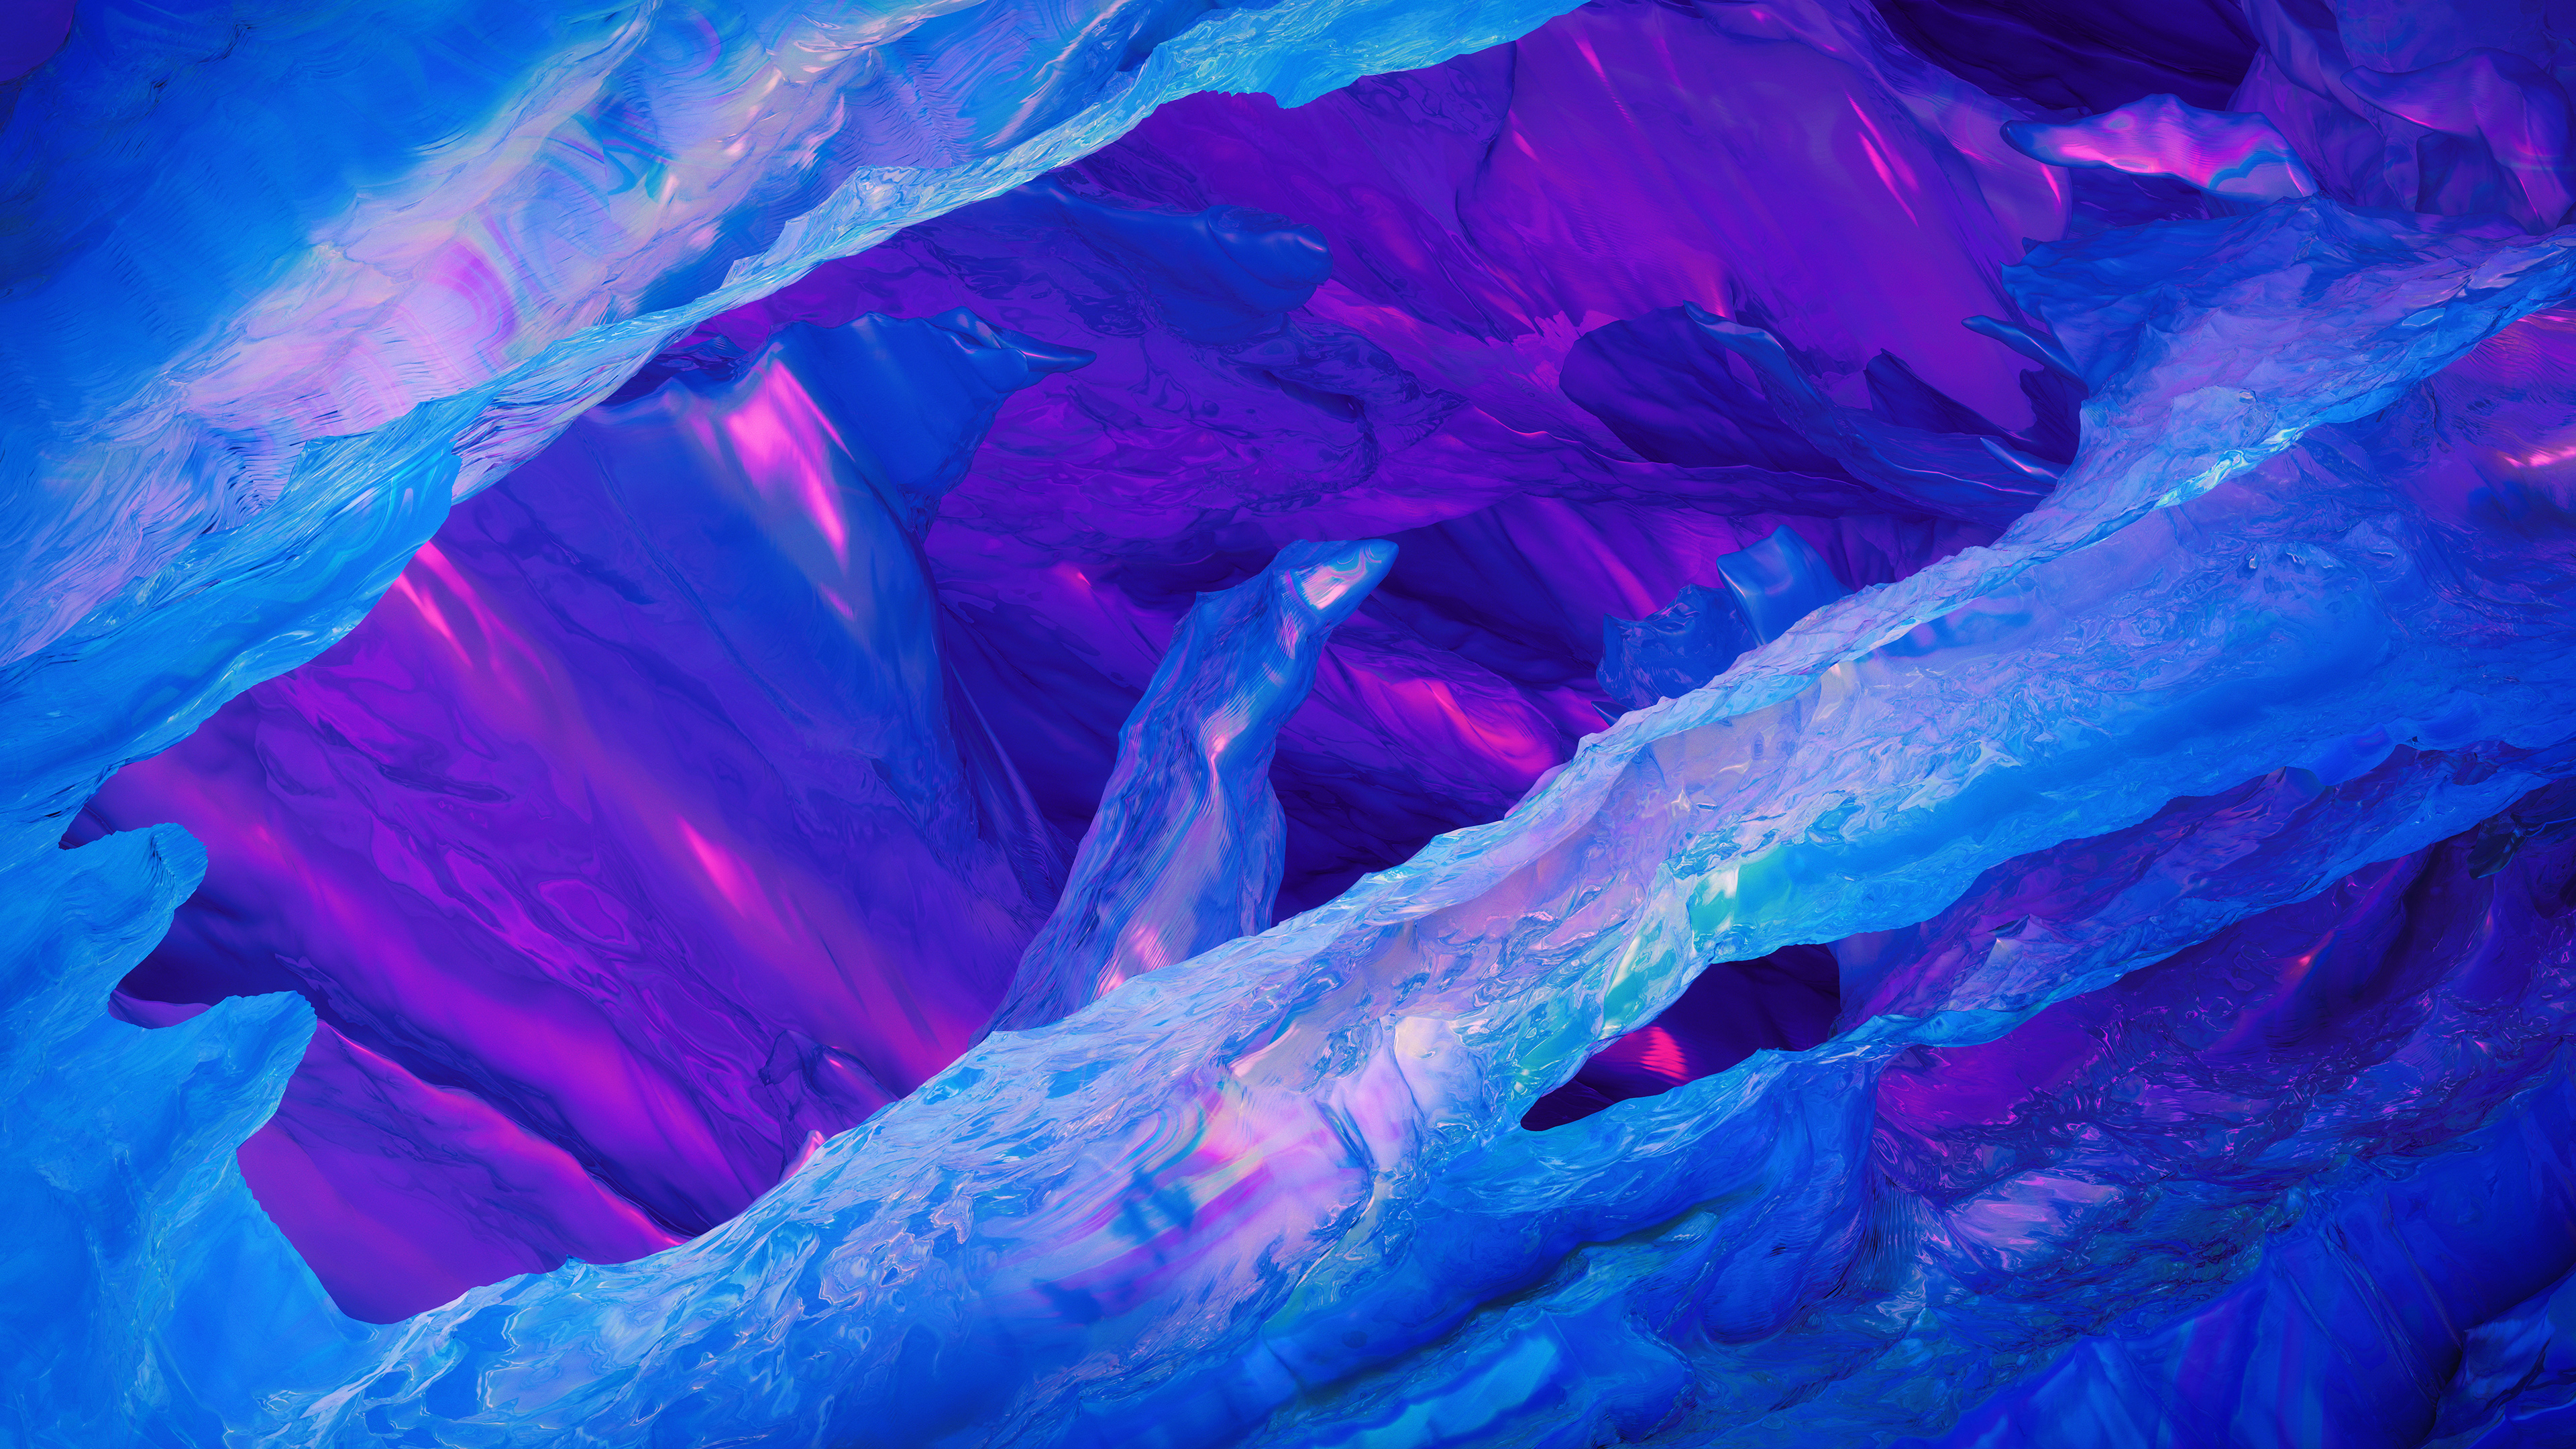
\includegraphics[scale=0.27]{./Imagens/9.png}
  \end{center}
  \legend{Fonte: O autor}
\end{figure}

Não houve período algum, entre a quarentena e o início das aulas
presenciais. Assim, o curso foi ministrado integralmente remoto.

\clearpage

\section{Definição dos temas do minicurso}

Todo o minicurso foi ministrado num modelo de
Ensino à Distância.

\subsection{Produção do Material Integral}

Durante o período de Agosto a Janeiro, desenvolveu-se as apresentações, e
uma apostila virtual, a qual contém material suplementar de estudo e
referência. A apostila foi disponibilizada por meio do
\href{https://github.com/26-55-87-BuddhiLW/MC-LaTeX}{repositório no
  GitHub}, e Google Clasroom, bem como materiais de apoio,
exemplos, e os modelos canônicos ABNT usados nas aulas.  Usou-se as
plataforma do Youtube, no canal da
\href{https://www.youtube.com/channel/UC9kL6UL-iEq4nJKGs1nezQQ}{LabEEL}
para disponibilizar as aulas à distância.

Com o software Krita, criou-se os planos de fundo que foram utilizados
pelo autor nas apresentações. Para isso, utilizou-se logos, e
logomarcas, da USP, da EEL, e do grupo LabEEL.


\subsection{Temas}

\setlist[enumerate]{noitemsep, lineskip=0pt}
\begin{enumerate}
\item Introdução, Filosofia, e Instalação do LaTeX - utilização de templates TeX.
\item Produção de Relatórios, Teses e Monografias, Sob Norma ABNT -
  pacote ABNTeX, imagens, tabelas, referências bibliográficas, e
  fórmulas matemáticas.
\item  Apresentações com pacote Beamer, citações ABNT - controle e modulação dos parâmetros de pacotes.
\end{enumerate}


A sequência é lógica, pois, não seria possível explicar a utilização de qualquer
pacote, sem o aluno saber o mínimo sobre a sintaxe da língua. Bem como, seria
misteriosa a escolha da língua, em relação a qualquer outro software tipográfico. Assim,
o primeiro item abordado foi a filosofia da linguagem e utilização de templates.
Desta forma, o aluno inicia a utilização da língua; entende seus porquês de ser,
e aprende a sintaxe básica a todo documento, escrito em \LaTeX.

Em seguida, o aluno já tem capacidade de se aprofundar na tipografia de documentos, sem muita
estilização específica. Por conseguinte, ensina-o a utilizar pacotes
essenciais a um estudante universitário - i.e., abntex2.

Por fim, as apresentações e autoformatação de citações foram
deixadas para a última aula. Porque, para serem compreendidas,
apresentam um nível superior de abstração em relação aos assuntos
supramencionados.

Ao concretizar-se o curso, o aluno adquiriu conhecimentos suficientes para entender, virtualmente, qualquer
pacote de \LaTeX{} mais complexo, ou modelos os quais utilizem muita
modulação, como seria o caso da produção de documentos como pôsteres.




\section{Divulgação}

No mês de fevereiro a partir do dia 17, utilizou-se de mídias sociais e de correspondência, como Facebook,
Whatsapp, e e-mail USP, para que os alunos sejam informados do curso,
bem como anunciar o período de inscrição. Escolheu-se o período de
divulgação com base nas datas de feriados e início de aulas.

Com o software Krita, criou-se uma arte conceptiva, para divulgação do
curso. Utilizou-se, para essa produção, do logo oficial do LabEEL.

A divulgação das aulas à distância, e mudança das  novas datas, foi feita no
período de Maio.

\section{Carga horária}
%% Para cada aula, foi alocada duas horas aula. Duas a quatro horas para se estudar
%% os materiais de cada módulo. E, duas a quatro horas para se completar cada lista
%% de exercício. Assim, o curso requeriria, no mínimo, 8 horas-crédito de dedicação para ser realizado.
Como o resultado foi de um abandono do curso foi menor do que 5\%, acredita-se que a carga horário foi coerente.

\section{Inscrição}
%% As inscrições seriam feitas por meio da internet, com a utilização do Google Forms.
%% Com esse recurso, coletaria-se número USP do aluno(a), telefone, e e-mail.

Houveram 80 inscritos. Assim, considera-se que o curso houve muitos inscritos, provando válida a maneira com que se fez as divulgações e os meios pelos quais se disponibilizou as inscrições.

\section{Avaliação}
%% Cada aula contaria com uma lista de exercícios, como método avaliativo. Desta forma,
%% haveriam três listas as quais contariam pela aprovação ou reprovação dos alunos.
Todo aluno que fez a primeira atividade terminou por fazer as demais. As avaliações tiveram notas foram altas; mais do que 80\% da nota total, em média. Isto pois os alunos apresentaram exatamente o que foi pedido nas litas de exercícios, com algumas exceções. As exceções se dão a não entrega total da lista, ou erros de interpretação do que foi pedido.

\section{Conclusão do Curso}

Na conclusão do curso, percebeu-se um entusiasmo grande dos alunos, em receberem seus certificados. E, houveram procuras posteriores dos alunos para se fazer da matéria. Esses dados estão de acordo com a teoria mais aceita da literatura, sobre motivação humana \cite{hendijani2016intrinsic}.

%% Ao fim do curso, seria dado ao aluno o qual completasse as listas um certificado
%% de participação e conclusão. Não se avisou os alunos sobre a gratificação, de
%% acordo com os conhecimentos e resultados decorrentes dos estudos de motivação
%% dos seres humanos \cite{deci2017self}. Fazer de outra maneira,
%% seria benéfico à participação das atividades \cite{hendijani2016intrinsic}.
%% Porém, detrimental ao desempenho posterior do aluno \cite{ariely2009large}.

\section{Participação dos Alunos}

Houveram 80 inscritos. Desses, 78 aceitaram o
convite de participação do Google Classroom. Apenas 22 alunos
completaram a primeira lista de exercícios, por mais que, todos que
fizeram, fizeram com excelência. Desses alunos, 20 fizeram a segunda
lista. E, por fim, a terceira lista foi feita por 19 alunos.

O resultado é compreensível, pois o curso exige muito do aluno, que
não está acostumado com programação. Outra coisa é que o curso não é
fácil, quem não está disposto, por
inclinações próprias, ou por não ter tempo suficiente, não iria
conseguir assistir às aulas, estudar o material, e completar as listas
de exercícios - dos quais eram simulações de situações recorrentes na
utilização do \LaTeX. Por conseguinte, observou um sucesso com os
objetivos do minicurso de capacitação, porém, houve uma distinção brusca entre as
partições dos alunos que se dedicaram integral às atividades, e os que
não.


\chapter{Conclusão}

O objetivo de capacitação de alunos da EEL-USP foi atingido. Porém,
com um decaimento expressivo de número de participantes ativos e
inscritos. Apenas 27.50\% dos alunos inscritos acometeu-se às atividades
do curso, de início; 23.75\%  completaram o curso. Assim, houve uma
desistência de 13.63\% dos participantes ativos. Isto é, \\
$\big(1-\frac{\text{(Alunos Completaram)\%}}{\text{(Alunos Inscritos
    Ativos)\%}} \big) \times 100\% = (1 - \frac{23.75\%}{27.50\%}) \times 100\% = 13.63\%$.

As listas possuíam uma complexidade coerente com os materiais e aulas
fornecidas. De forma que, se o aluno completasse as listas, seria
possível, seguramente, que o aluno conseguisse integrar o uso da
ferramenta na produção de documentos, no seu dia a dia. Pois, todos os
exercícios foram tirados de situações reais, do qual o autor
enfrentou, em seu caminho acadêmico na faculdade.



\bibliography{bib}


\end{document}

%%% Local Variables:
%%% mode: latex
%%% TeX-master: t
%%% End:
